\chapter{Технологическая часть}

В данной части рассматривается выбор средств реализации, описывается структура классов программы и приводится интерфейс программного обеспечения.

\section{Средства реализации}
В данной работе для реализации был выбран язык программирования $C\#$ [7].

Для разработки интерфейса и работы с пикселями изображения была выбрана платформа $Windows Forms$ [8].

Выбор обусловлен наличием стандартной библиотеки для работы с векторами и матрицами ($System.Numerics$) и библиотеки для работы с графикой ($System.Drawing$). Используемые инструменты обладают полным функционалом для разработки, профилирования и отладки необходимой программы. 

\section{Структура программы}
Разработанная программа состоит из следующих классов. Математические классы:
\begin{itemize}
    \item[$-$] Vector3D $-$ класс для работы с трехмерными векторами;
    \item[$-$] Matrix4x4 $-$ класс для работы с матрицами 4x4.
\end{itemize}

Классы для работы с моделями:
\begin{itemize}
    \item[$-$] Mesh $-$ класс, представляющий трехмерную модель;
    \item[$-$] Vertex $-$ класс, представляющий вершину;
    \item[$-$] Face $-$ класс, представляющий полигон (треугольник) в сетке;
    \item[$-$] Indentation $-$ класс, представляющий лунку (углубление) на поверхности.
\end{itemize}

\clearpage
Вспомогательные классы:
\begin{itemize}
    \item[$-$] Camera $-$ класс, представляющий камеру;
    \item[$-$] Light $-$ класс, представляющий источник света;
    \item[$-$] Scene $-$ класс, представляющий сцену;
    \item[$-$] Form $-$ класс, представляющий интерфейс.
\end{itemize}

На рисунке~\ref{fig:uml} представлена диаграмма разработанных классов.

\begin{figure}[H]
    \centering
    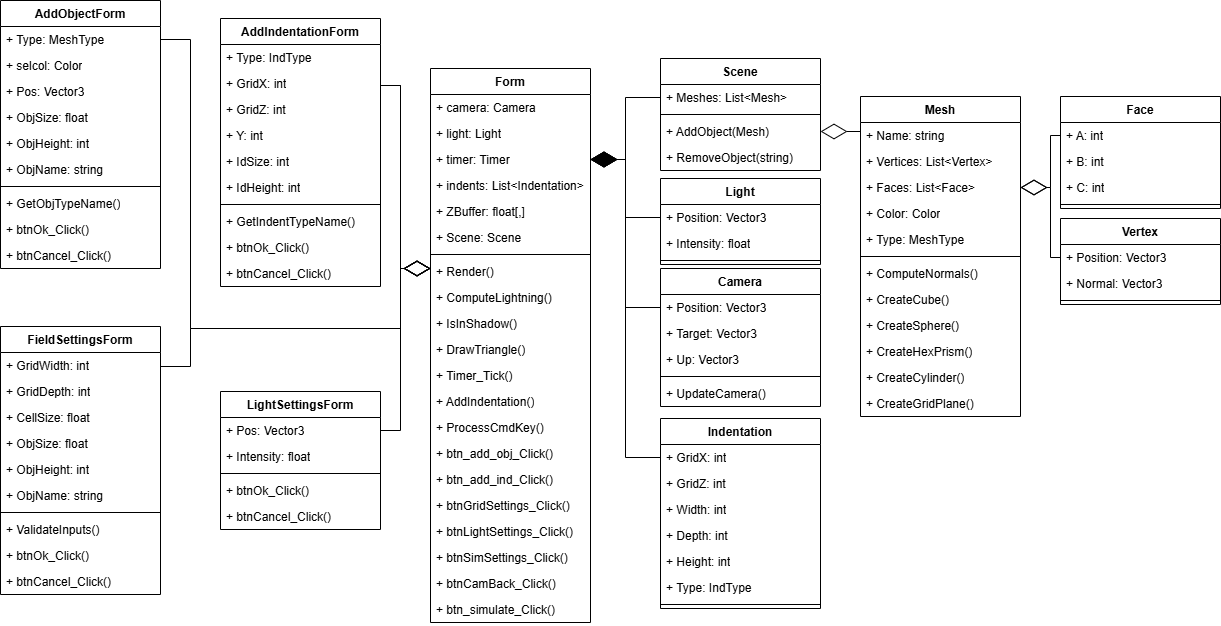
\includegraphics[width=1\linewidth]{img/CG_CP.drawio.png}
    \caption{Диаграмма классов программы}
    \label{fig:uml}
\end{figure}

\section{Схемы алгоритмов}

% В листингах \ref{lst:zbuf} $-$ \ref{lst:shadow} представлены реализации алгоритмов.
Схемы алгоритмов представлены на рисунках~\ref{fig:z}$-$~\ref{fig:shadow}.
\clearpage
\begin{figure}[h!]
    \centering
    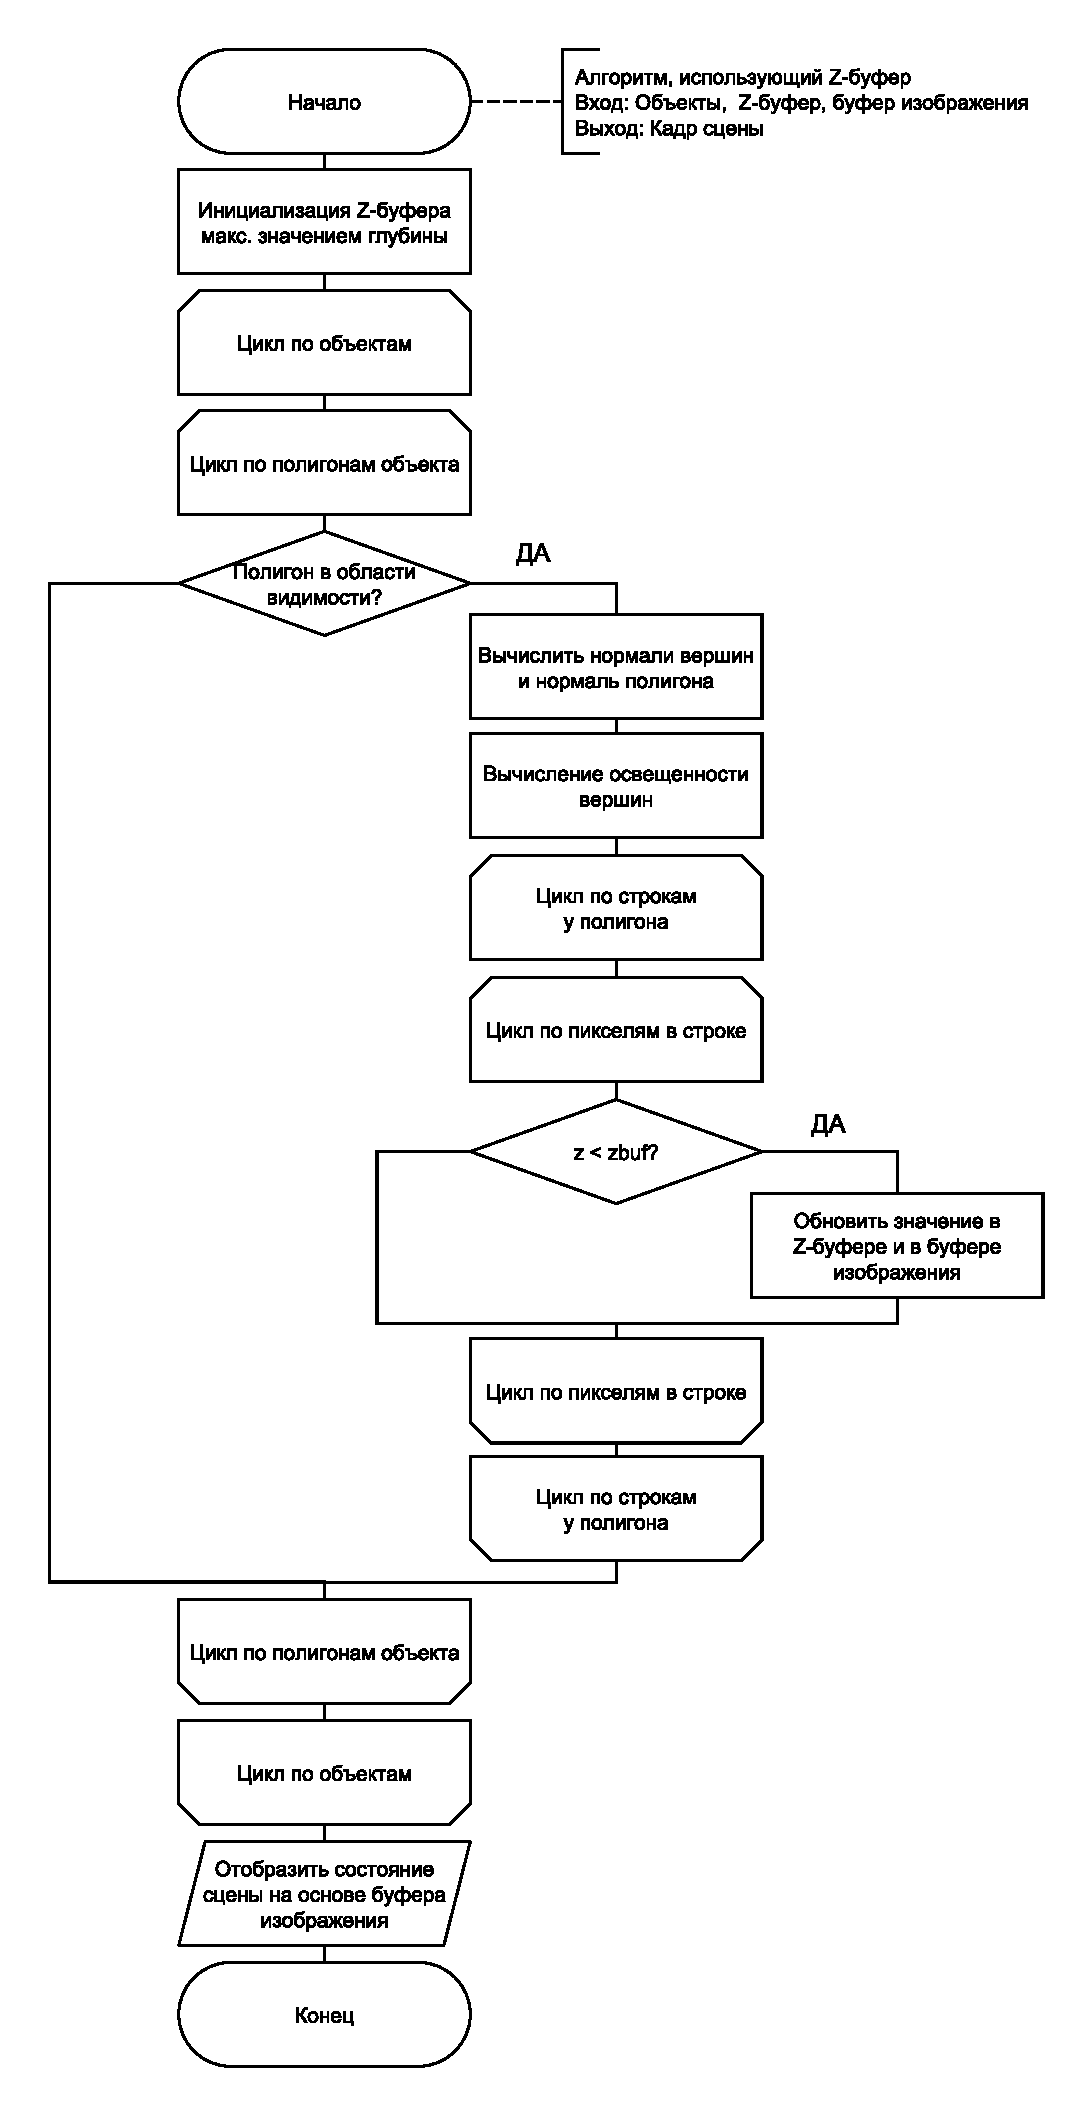
\includegraphics[scale=0.65]{img/zbuf.eps}
    \caption{Схема алгоритма, использующего Z-буфер}
    \label{fig:z}
\end{figure}
\begin{figure}[h!]
    \centering
    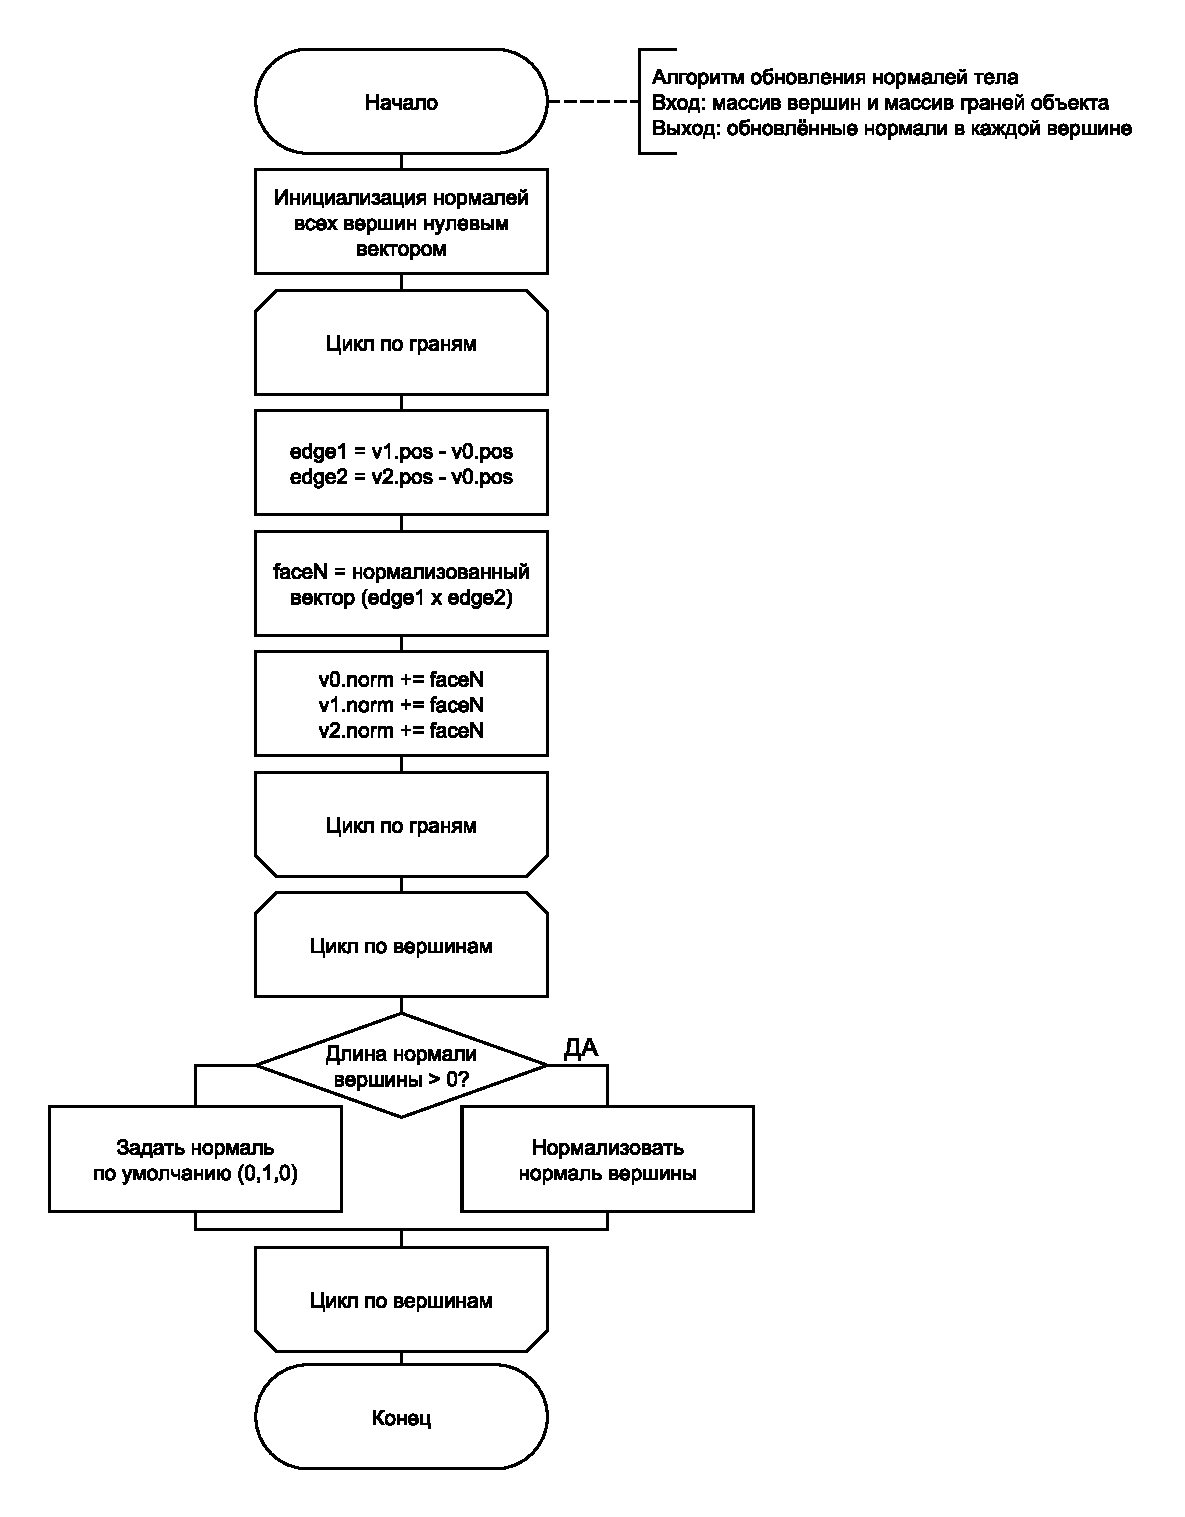
\includegraphics[scale=0.45]{img/normals.eps}
    \caption{Схема алгоритма обновления нормалей объекта}
    \label{fig}
\end{figure}
\begin{figure}[h!]
    \centering
    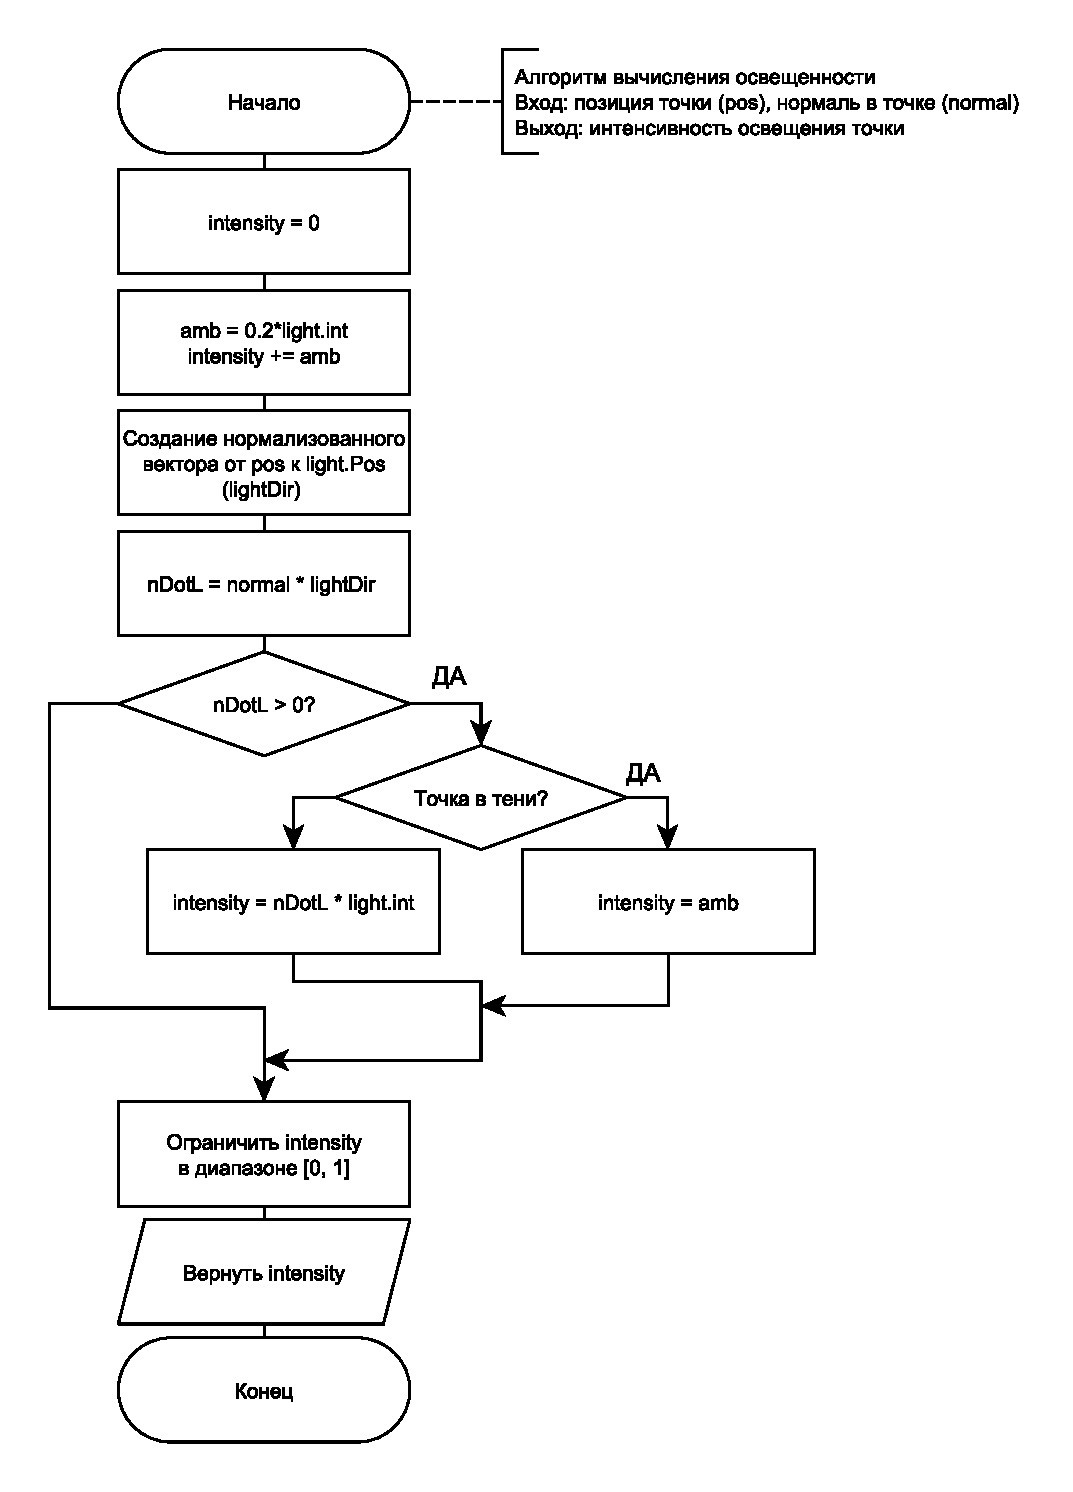
\includegraphics[scale=0.45]{img/computelight.eps}
    \caption{Схема алгоритма вычисления освещенности}
    \label{fig}
\end{figure}
\begin{figure}[h!]
    \centering
    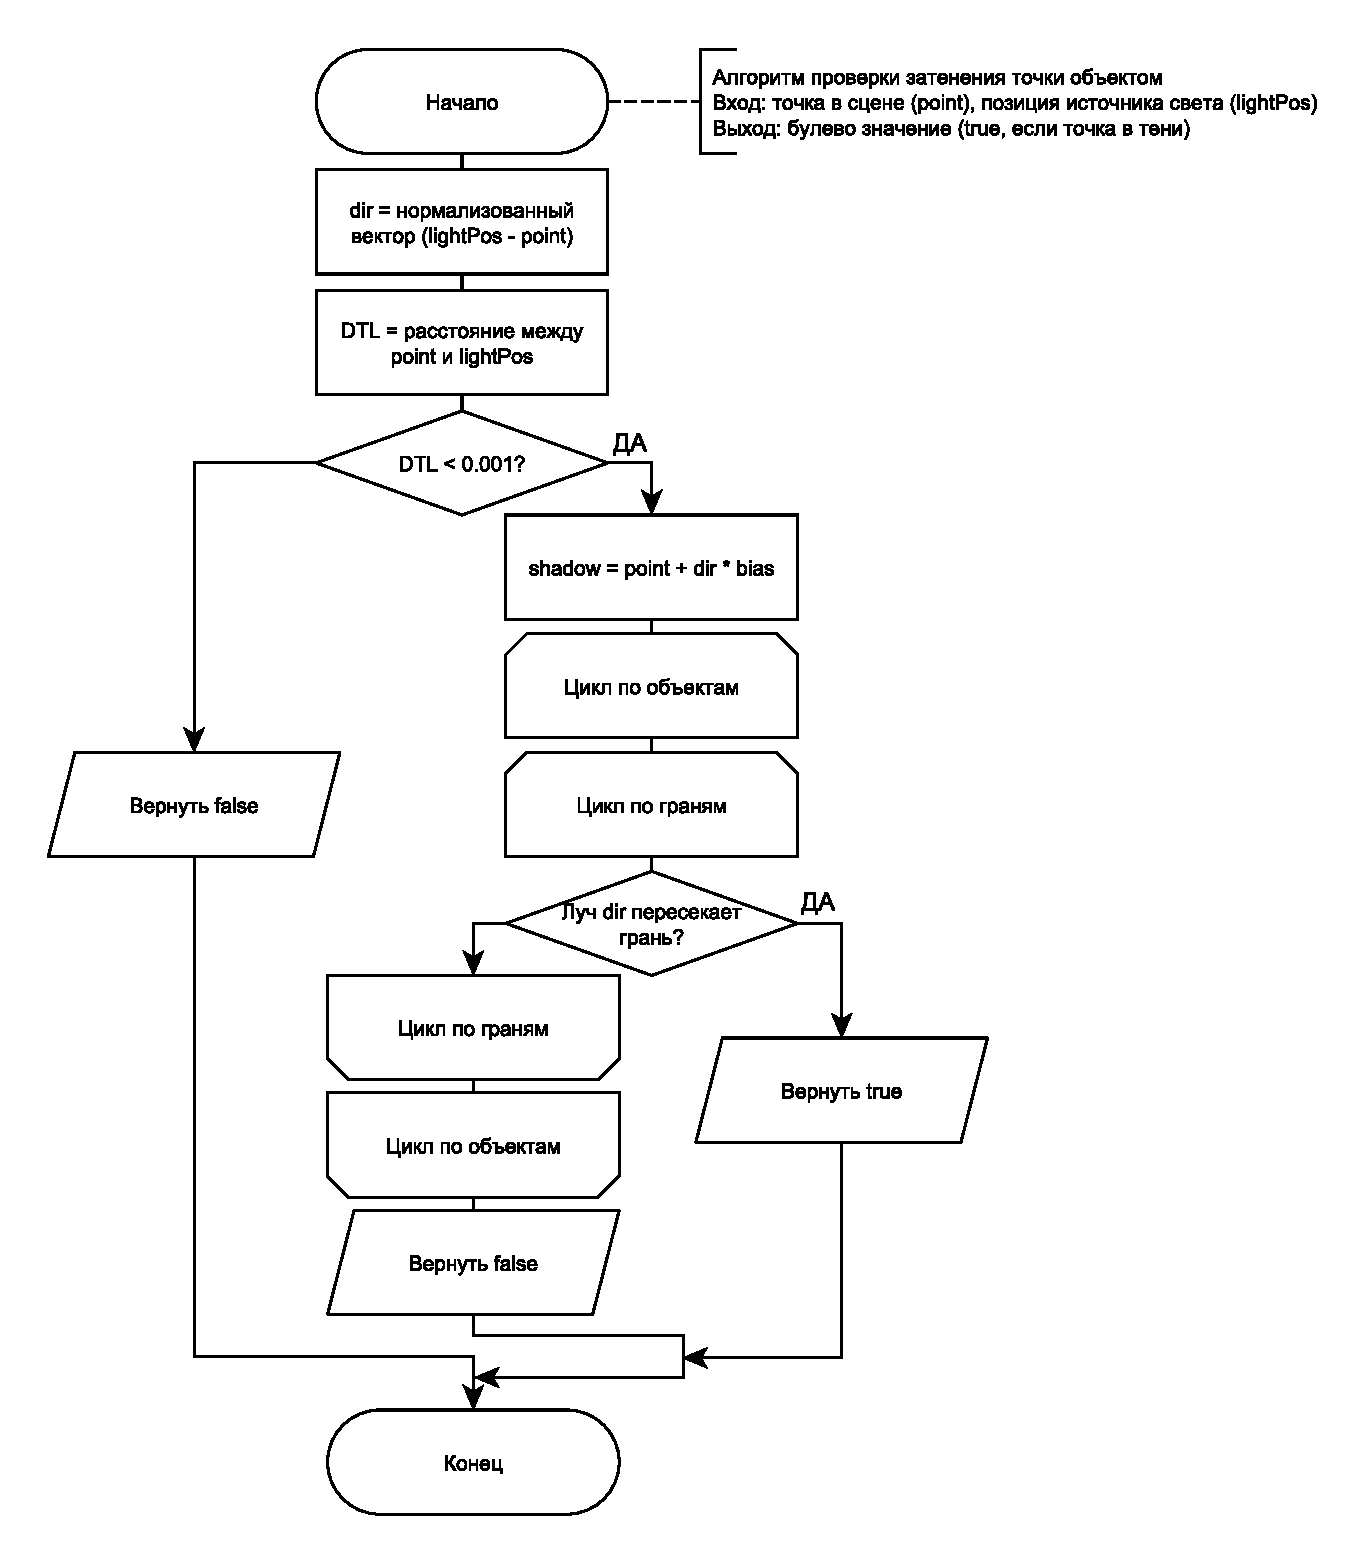
\includegraphics[scale=0.5]{img/shadow.eps}
    \caption{Схема алгоритма проверки затенения точки объектом}
    \label{fig:shadow}
\end{figure}


\vspace{5mm}

\section{Интерфейс программного обеспечения}
\begin{figure}[h!]
    \centering
    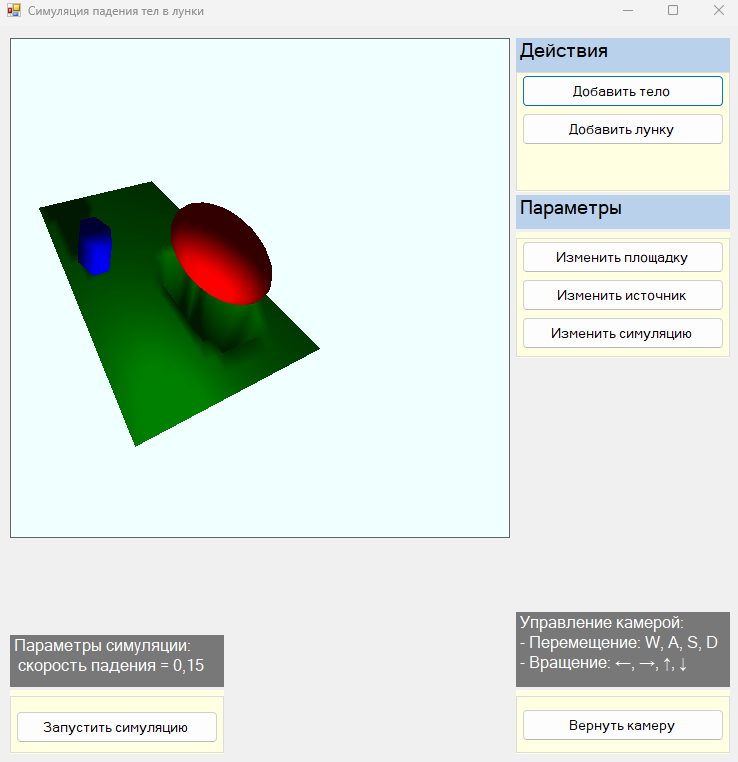
\includegraphics[width=0.4\linewidth]{img/int-1-2.png}
    \caption{Графический интерфейс программы}
    \label{fig:int-1}
\end{figure}

Главное окно программы представлено на рисунке~\ref{fig:int-1}. При запуске программы в левой части определен компонент сцены, в правой части определены компоненты, отвечающие за изменение тел, лунок и параметров площадки, источника света и симуляции. В нижней части описаны правила пользования камерой, а также опеределена кнопка запуска симуляции с указанной скоростью падения.

Для создания тела пользователю необходимо в главном меню нажать кнопку «Добавить тело» и в появившемся окне указать все нужные параметры (рисунок~\ref{fig:int-2}).


\begin{figure}[h!]
    \centering
    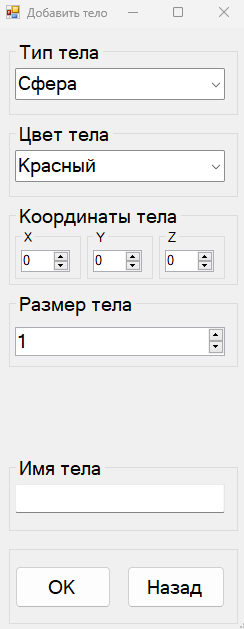
\includegraphics[width=0.15\linewidth]{img/int-2.png}
    \caption{Параметры тела}
    \label{fig:int-2}
\end{figure}

Для создания лунки пользователю необходимо в главном меню нажать кнопку «Добавить лунку» и в появившемся окне указать все нужные параметры (рисунок~\ref{fig:int-3}).

\begin{figure}[h!]
    \centering
    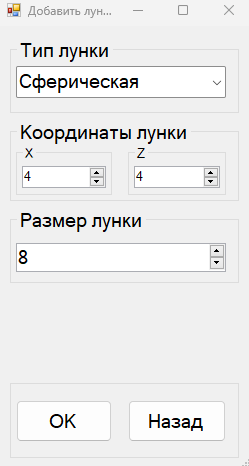
\includegraphics[width=0.15\linewidth]{img/int-3.png}
    \caption{Параметры лунки}
    \label{fig:int-3}
\end{figure}

Для изменения площадки пользователю необходимо в главном меню нажать кнопку «Изменить площадку» и в появившемся окне указать размер клетки и количество клеток в длину и в ширину (рисунок~\ref{fig:int-4}).

\begin{figure}[h!]
    \centering
    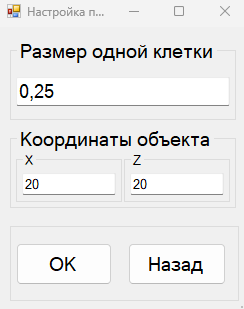
\includegraphics[width=0.15\linewidth]{img/int-4.png}
    \caption{Параметры площадки}
    \label{fig:int-4}
\end{figure}

Для изменения параметров источника света пользователю необходимо в главном меню нажать кнопку «Изменить источник» и в появившемся окне указать положение источника и его интенсивность (рисунок~\ref{fig:int-5}).

\begin{figure}[h!]
    \centering
    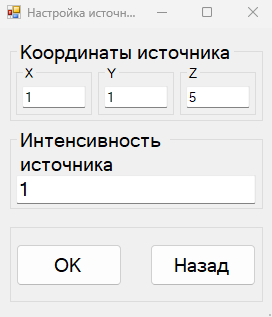
\includegraphics[width=0.15\linewidth]{img/int-5.png}
    \caption{Параметры источника света}
    \label{fig:int-5}
\end{figure}

Для изменения скорости падения объектов необходимо в главном меню нажать кнопку «Изменить симуляцию» и в появившемся окне указать скорость падения объектов (рисунок~\ref{fig:int-6}).

\begin{figure}[h!]
    \centering
    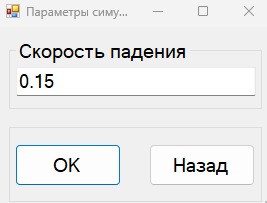
\includegraphics[width=0.15\linewidth]{img/int-6.png}
    \caption{Параметры симуляции}
    \label{fig:int-6}
\end{figure}


\textbf{ВЫВОД}

В данном разделе были выбраны средства реализации, описаны структуры классов программы, описаны модули, а также рассмотрен интерфейс
программы.

\clearpage